\documentclass[draft,final]{vutinfth} % Remove option 'final' to obtain debug information.
% Load packages to allow in- and output of non-ASCII characters.
\usepackage{lmodern}        % Use an extension of the original Computer Modern font to minimize the use of bitmapped letters.
\usepackage[T1]{fontenc}    % Determines font encoding of the output. Font packages have to be included before this line.
\usepackage[utf8]{inputenc} % Determines encoding of the input. All input files have to use UTF8 encoding. % Extended LaTeX functionality is enables by including packages with
\usepackage{amsmath}    % Extended typesetting of mathematical expression.
\usepackage{amssymb}    % Provides a multitude of mathematical symbols.
\usepackage{mathtools}  % Further extensions of mathematical typesetting.
\usepackage{microtype}  % Small-scale typographic enhancements.
\usepackage[inline]{enumitem} % User control over the layout of lists (itemize, enumerate, description).
\usepackage{multirow}   % Allows table elements to span several rows.
\usepackage{booktabs}   % Improves the typesettings of tables.
\usepackage{subcaption} % Allows the use of subfigures and enables their referencing.
\usepackage[ruled,linesnumbered,algochapter]{algorithm2e} % Enables the writing of pseudo code.
\usepackage[usenames,dvipsnames,table]{xcolor} % Allows the definition and use of colors. This package has to be included before tikz.
\usepackage{nag}       % Issues warnings when best practices in writing LaTeX documents are violated.
\usepackage{todonotes} % Provides tooltip-like todo notes.
\usepackage{hyperref}  % Enables cross linking in the electronic document version. This package has to be included second to last.
\usepackage[acronym,toc,nomain]{glossaries} % Enables the generation of glossaries and lists fo acronyms. This package has to be included last. % Define convenience functions to use the author name and the thesis title in the PDF document properties.

\usepackage{fancyvrb}
\usepackage{cite}
\usepackage{graphicx}
\usepackage[section]{placeins}

\newcommand{\authorname}{Jakob Fischer} % The author name without titles.
\newcommand{\thesistitle}{Case Study on an Elektra storage plugin} % The title of the thesis. The English version should be used, if it exists. 

\hypersetup{
	pdfpagelayout   = TwoPageRight,           % How the document is shown in PDF viewers (optional).
	linkbordercolor = {Melon},                % The color of the borders of boxes around crosslinks (optional).
	pdfauthor       = {\authorname},          % The author's name in the document properties (optional).
	pdftitle        = {\thesistitle},         % The document's title in the document properties (optional).
	pdfsubject      = {Subject},              % The document's subject in the document properties (optional).
	pdfkeywords     = {a, list, of, keywords} % The document's keywords in the document properties (optional).
}

\setpnumwidth{2.5em}        % Avoid overfull hboxes in the table of contents (see memoir manual).
\setsecnumdepth{subsection} % Enumerate subsections.

\nonzeroparskip             % Create space between paragraphs (optional).
\setlength{\parindent}{0pt} % Remove paragraph identation (optional).

\makeindex      % Use an optional index.
\makeglossaries % Use an optional glossary.

% Set persons with 4 arguments:
%  {title before name}{name}{title after name}{gender}
%  where both titles are optional (i.e. can be given as empty brackets {}).
\setauthor{}{\authorname}{}{male}
\setadvisor{Dr.techn. Dipl.-Ing.}{Markus Raab}{}{male}

% For bachelor and master theses:
% \setfirstassistant{Pretitle}{Forename Surname}{Posttitle}{male}

% Required data.
\setregnumber{01427178}
\setdate{27}{11}{2019}
\settitle{\thesistitle}{Viability of TOML parsing for configuration}

% Select the thesis type: bachelor / master / doctor / phd-school.
% Bachelor:
\setthesis{bachelor}

% For bachelor and master:
\setcurriculum{Software and Information Engineering}{Software und Information Engineering} % Sets the English and German name of the curriculum.

\title{Case Study on an Elektra storage plugin }
\author{Jakob Fischer}

\bibliographystyle{unsrt}

\newacronym{ll}{LL}{Left-to-Right, Leftmost derivation}
\newacronym{lr}{LR}{Left-to-Right, Rightmost derivation in reverse}
\newacronym{toml}{TOML}{Tom's Obvious, Minimal Language}
\newacronym{yaml}{YAML}{YAML Ain't Markup Language}
\newacronym{ini}{INI}{Initalization}
\newacronym{flex}{Flex}{Fast Lexical Analyzer}
\newacronym{posix}{POSIX}{Portable Operating System Interface}
\newacronym{tmux}{tmux}{Terminal Multiplexer}
\newacronym{lcd}{LCD}{Liquid Crystal Display}
\newacronym{api}{API}{Application Programming Interface}
\newacronym{floss}{FLOSS}{Free/Libre/Open Source Software}

\newcommand{\onlinesrc}[1]{Accessed #1}
\newcommand{\gitsrc}[1]{Commit \##1}

\begin{document}

\frontmatter

\addtitlepage{english}
\addstatementpage

% \begin{acknowledgements*}
% \end{acknowledgements*}

% \begin{kurzfassung}
% \todo{KURZFASSUNG HIER}
% \end{kurzfassung}


\begin{abstract}
Elektra is a library for handling configuration data, which also can mount external configuration files into it's system with the help of storage plugins.
These storage plugin convert the file specific format into Elektra's format.
As part of this thesis, we wrote such a storage plugin, for enabling the usage of \acrshort{toml} configuration files within Elektra.
We evaluated the written plugin on the \acrshort{floss} project LCDproc, where we checked, if the plugin correctly reads and writes the configuration.
Additionally, we compared the reading speed of our plugin with two other existing storage plugins within LCDproc.
The newly written plugin could read and write \acrshort{toml} configuration without any loss of information.
It's reading speed of \acrshort{toml} files was as good as the two other plugins, we matched it against.
\end{abstract}

\selectlanguage{english}

\tableofcontents

\mainmatter

\chapter{Introduction}

The practical part of this thesis consisted of writing an Elektra storage plugin, which can handle the reading and writing of \acrshort{toml} (\acrlong{toml}) configuration files from and into the key database Elektra handles.

\section{\acrshort{toml}}
\acrlong{toml} is a configuration file format developed since February 2013 \cite{tomlcontrib}.
It claims to be a format that is easily to read and parse \cite{tomlreadme} and finds use in many different projects \cite{tomlwiki}, such as Rust's project manager \texttt{cargo} \cite{cargogit} or Python's package installer \texttt{pip} \cite{piprefguide}.

\section{Elektra}
Elektra is a configuration framework for accessing configuration settings in a global key database \cite{elektramain}.
An application using Elektra can read and write key/value pairs via calls to the Elektra library, making the implementation of an own configuration system obsolete.
Furthermore, elektrified applications can access each others configuration settings, to provide better application interoperability.

Although Elektra is mainly written in C, there are bindings for other languages like java, python or ruby \cite{elektrabindings}.

Elektra can also read from and write to different configuration file formats, like JSON, XML or ini \cite{elektrastorage}.
When needed, applications can easily switch to a different file format, because configuration access is done with the Elektra \acrshort{api}.
Developers or Administrators no longer have to commit to one file format for configuration.

Support for different languages and file formats is implemented by the use of plugins, which can be enabled if necessary.
With this modularity, Elektra can provide a wide range of functionality, while simultaneously avoiding being a bloated library.
Developers can compile Elektra with the exact set of needed functionality.

\section{LCDproc}
LCDproc is an open source project for displaying stats like CPU/RAM usage of a system on different kinds of \acrshort{lcd} (\acrlong{lcd}) devices \cite{lcdprocmain}\cite{lcdprocgit}.
It has a client/server architecture, where the clients provide their system stats to the server, which can display them on a \acrshort{lcd} device.

\section{Research Question}
As part of this thesis, we wrote an Elektra storage plugin for reading and writing \acrshort{toml} files.
We will test this newly written \acrshort{toml} plugin on ElektraInitiative's fork of LCDproc, where it gets modified to use Elektra for it's handling of configuration.
The \acrshort{toml} plugin will be used as the storage plugin for the LCDproc configuration.
For evaluation, \acrshort{toml} configuration files for each tested part of LCDproc were created.

There are three questions we want to answer for the \acrshort{toml} plugin:
\begin{itemize}
	\item[\textbf{RQ1}] Does the plugin correctly read the LCDproc configuration?
	\item[\textbf{RQ2}] Does the plugin correctly write the LCDproc configuration without any loss of information?
	\item[\textbf{RQ3}] Does the plugin put an unreasonable overhead on LCDproc loading times?
\end{itemize}
When answering RQ1, we also must ensure that we are reading the configuration from our supplied file, and not the default values supplied by the Elektra specification.

Ad RQ2 we also have to check, if comments and newlines - which don't affect the LCDproc execution practically, but are only for the user to read - are preserved.

\chapter{Implementation}

The plugin is implemented in C, using the C99 standard. It requires \acrshort{posix} for some checks using regular expressions.

\section{Plugin}
The \acrshort{toml} parser is realized as an Elektra storage plugin. The plugin exposes two functions, \textbf{ElektraTomlGet} for reading, and \textbf{ElektraTomlSet} for writing, as expected of an Elektra storage plugin.

\section{Tools}
It uses two external tools for generating a parser for the toml file format: \textbf{\acrshort{flex}} (\acrlong{flex}) \cite{flexgit} for lexical analysis and \textbf{bison} \cite{bisonmain} for parsing.
The key generation is done in the bison parser with the use of actions.

In order to generate the appropriate Elektra keys, the parser has access to a driver, which contains all needed Elektra logic.
We adapted this driver oriented approach from the \textbf{yambi}\cite{Elektrayambi} plugin.
The driver contains functions int the style of \\ \texttt{driverEnterKey}/\texttt{driverExitTable}, to clarify, on which point of parsing a certain function shall be invoked.

\section{Grammar}
Since bison generates \acrshort{lr} (\acrlong{lr}) parsers, grammar rules should be left-recursive.
Otherwise, when using right-recursive rules, the parser would first need to shift the whole recursive expression onto the stack before it can start reducing it.
The parser could run out of stack space, if it must parse right-recursive rules too deep, as it may happen when parsing a huge array.
Therefore, the written parser only contains left-recursive rules.

The parser makes use of so-called midrule-actions, which are parser actions that are not placed at the end of a grammar rule.
This can affect the resulting grammar, since after executing a mid-rule action, the parser has to commit to the chosen parse branch \cite{bisonmidruleconflicts}.
We tried to minimize the usage of midrule-actions, to make the grammar as independent of actions as possible.
However, especially for possibly nested structures like arrays or inline tables they were unavoidable.

\chapter{Methodology}
In this evaluation, we will check four parts of LCDproc: The server daemon \texttt{LCDd} and three clients, namely \texttt{lcdproc}, \texttt{lcdexec}, \texttt{lcdvc}.
To valid the way, the \acrshort{toml} plugin reads/writes configuration, we will force a roundtrip of the file by changing a value within that file with the Elektra command \texttt{kdb set}.
When we call \texttt{kdb set}, the configuration first gets read from the file, the value to set is updated, and then the keys are written back into the file.
After we roundtripped a file, we compare it with its original file by the help of the \texttt{diff} command.
This \texttt{diff} command is always invoked with the \texttt{-w} switch, so that whitespace differences get ignored.
The \acrshort{toml} plugin currently preserves whitespace only before comments (tabs get converted into four spaces).

The \acrshort{toml} files copied during installation either differ from the default configuration loaded by the specification, or we will alter the keys of the file by a call of \texttt{kdb set} before we execute the program.
During execution, we check if the program starts without any errors concerning the reading of the \acrshort{toml} file.
We also check, if we can observe the expected difference from the default configuration, to ensure that we really are using the values from our configuration file.

In order to check, if the plugin imposes an unreasonable overhead in the loading times of LCDproc, we conducted benchmarks.
There, we compared the loading time of LCDproc while using the existing storage plugins yamlcpp, ni and our \acrshort{toml} for loading configuration.


\chapter{Evaluation}

\section{Hardware Setup}
The evaluation was executed on the following hardware setup:
\begin{Verbatim}[frame=single]
Processor: Intel i7-4790K @ 4.20 GHz
RAM: 16 GB (2 x 4GB, 1 x 8GB), DDR-3 @ 1600 MHz 
HDD: Seagate Desktop ST2000DM001, 2TB, 6 GB/s
\end{Verbatim}

\section{Software Setup}

The following versions of Elektra and LCDproc were used for evaluation:
\begin{Verbatim}[frame=single]
Elektra:
repository: github.com/bauhaus93/libelektra.git
branch: 'plugin_toml'
commit: #6de556aea56f556c4bdd208394b98974565cb1e9
LCDproc:
repository: github.com/bauhaus93/lcdproc.git
branch: 'toml_test'
commit: #0660eed82246b71b93b7d2e485b5620fa404b010
\end{Verbatim}


The evaluation was done within a docker container, which was built as follows.
\begin{Verbatim}[frame=single]
cd libelektra
docker build -t buildElektra-buster \
    --build-arg JENKINS_USERID=`id -u` \
    --build-arg JENKINS_GROUPID=`id -g` \
    -f scripts/docker/debian/buster/Dockerfile \
    scripts/docker/debian/buster/
\end{Verbatim}

We extended this image by building another image on top of it. This dockerfile mainly installs/sets up sudo for installing Elektra and LCDproc.
\begin{Verbatim}[frame=single]
FROM buildelektra-buster
USER root
RUN apt-get update && apt-get -y install sudo vim tmux
RUN adduser jenkins sudo
RUN echo '%sudo ALL=(ALL) NOPASSWD:ALL' >> /etc/sudoers
USER jenkins
WORKDIR /home/jenkins
\end{Verbatim}

As a last step, we invoke a setup script. It installs Elektra and LCDdproc, and then copies LCDproc \acrshort{toml} files to the \texttt{./config} directory.
\begin{Verbatim}[frame=single]
./lcdproc/toml_setup_install.sh
\end{Verbatim}
This script also invokes the \texttt{post-install.sh} script, which will mount the configuration scripts at the point expected by LCDproc.

\section{LCDd}
The LCDd server displays stats sent by the client applications to \acrshort{lcd} displays.
For our purposes, we configured it to display it to curses.
Since the default configuration LCDd file is very minimal, and most of the configuration is loaded by the specification, we created a LCDd \acrshort{toml} file for evaluation purposes.
It is based on the old default configuration file of LCDd \cite{LCDprocconf}.
We converted this old configuration from it's ini-like format into \acrshort{toml}.
All driver configuration settings, which are not referenced in the specification \cite{bauhausforklcdprocslcddspec}, were removed.

The resulting \acrshort{toml} file has 606 lines including 369 lines of comments and 143 empty lines.
It contains a table and a nested array.
It also contains multiple \acrshort{toml} table arrays - one for each LCDproc driver.

We force a full read/write roundtrip of the configuration file by setting the currently used driver. This driver is already the active one in the file, but we just set it again for the roundtrip.
Afterwards, we check if there are any differences between the original file and the newly written file.

\begin{Verbatim}[frame=single, fontsize=\small]
kdb set '/sw/lcdproc/lcdd/#0/current/server/drivers/#0' '@/curses/#0'
diff -ws ./lcdproc/LCDd.toml .config/LCDd.toml
Files ./lcdproc/LCDd.toml and .config/LCDd.toml are identical
\end{Verbatim}

After the roundtrip, the resulting LCDd.toml is identical to the original file under disregard of whitespace.
\\\\
We start and stop the LCDd daemon once, change some parameters of the curses driver, and start the daemon again.
\begin{Verbatim}[frame=single, fontsize=\small]
LCDd -f
kdb set '/sw/lcdproc/lcdd/#0/current/curses/#0/foreground' 'yellow'
kdb set '/sw/lcdproc/lcdd/#0/current/curses/#0/background' 'blue'
kdb set '/sw/lcdproc/lcdd/#0/current/curses/#0/backlight' 'blue'
kdb set '/sw/lcdproc/lcdd/#0/current/curses/#0/size' '100x40'
LCDd -f
\end{Verbatim}

The resulting output of LCDd is:
\FloatBarrier
\begin{figure}[!ht]
	\centering
	\begin{subfigure}[b]{0.4\linewidth}
		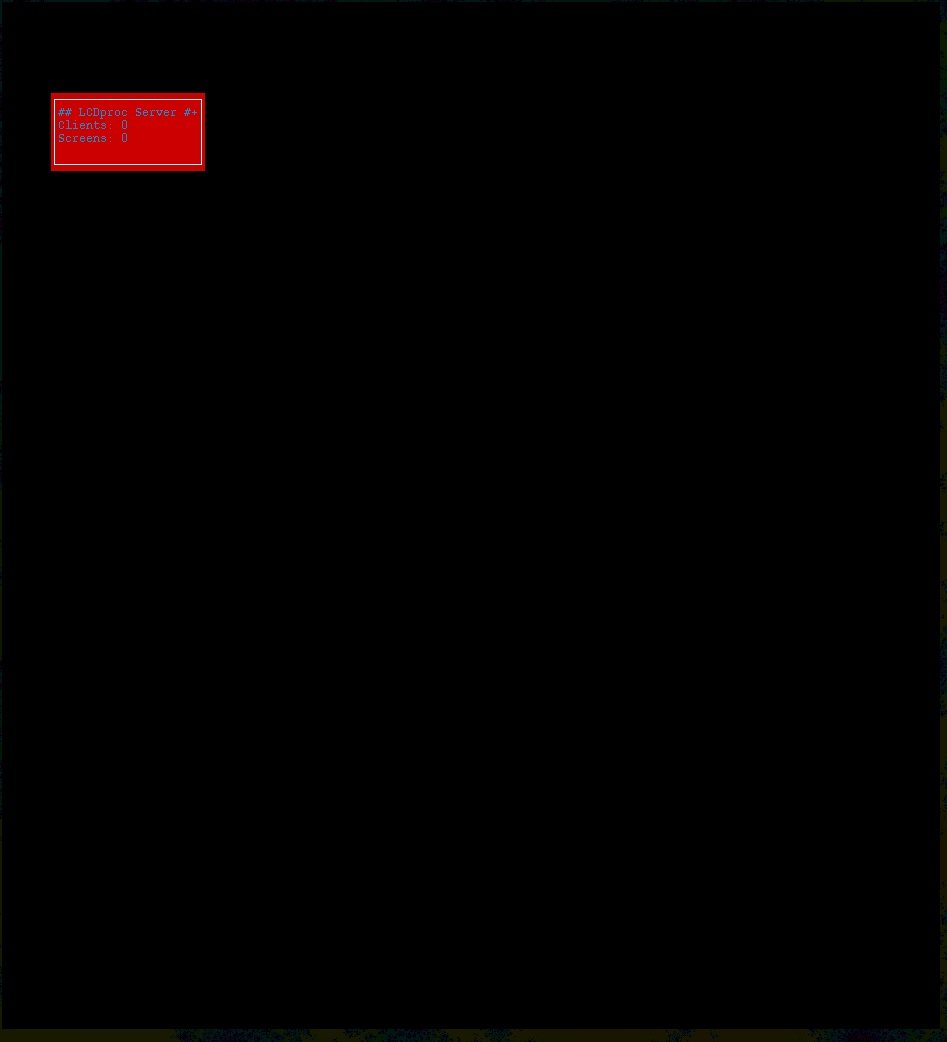
\includegraphics[width=\linewidth]{graphics/lcdd_vanilla.png}
		\caption{Before parameter change}
	\end{subfigure}
	\begin{subfigure}[b]{0.4\linewidth}
		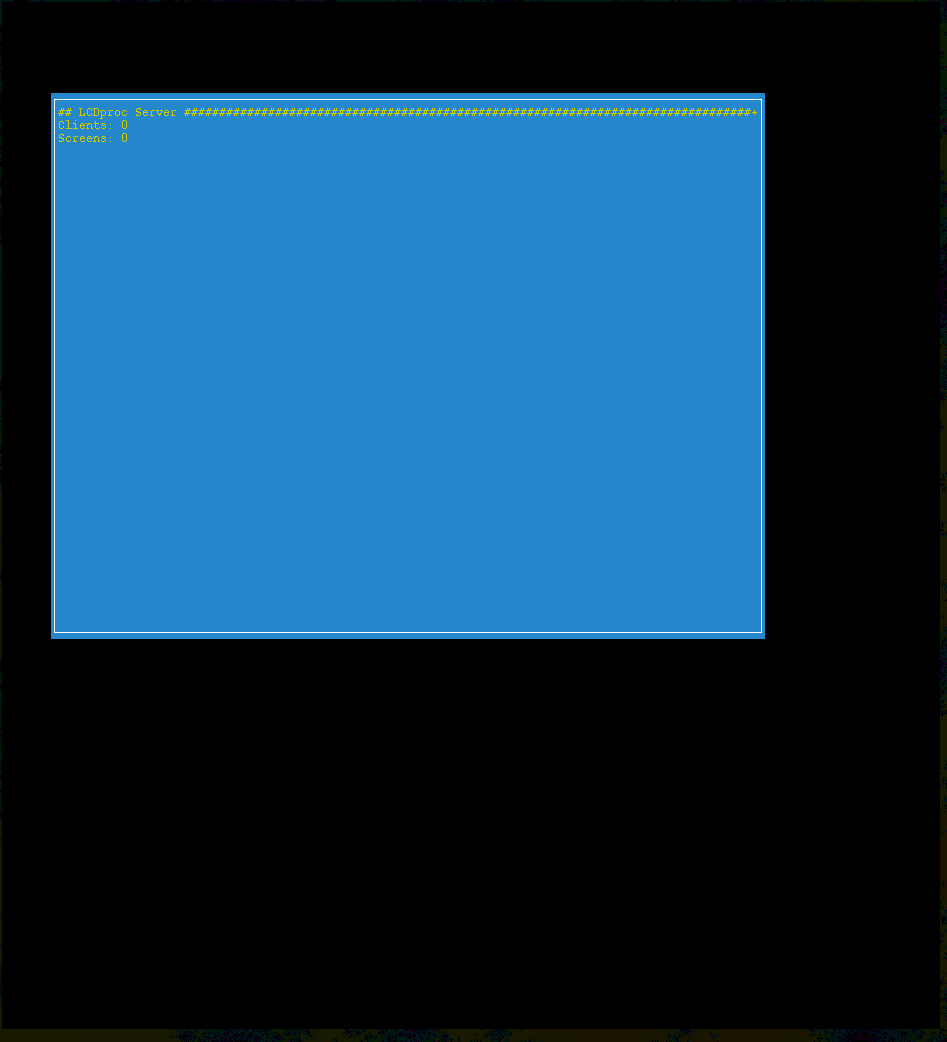
\includegraphics[width=\linewidth]{graphics/lcdd_changed.png}
		\caption{After parameter change}
	\end{subfigure}
  \caption{LCDd output}
\label{fig:lcdd}
\end{figure}
\FloatBarrier
We observe, that we successfuly changed the foreground/background color and window size of the daemon.

\section{lcdproc}
The lcdproc client is the main client for LCDproc. It sends the stats of it's host to the connected LCDd server.
The configuration file used for the evaluation of lcdproc contains has 156 lines, including 58 lines of comment and 46 empty lines.
The lcdproc configuration gets roundtripped by changing the used port from the default value of 13666 to 12345.
Afterwards the file difference without whitespace gets checked.
\begin{Verbatim}[frame=single, fontsize=\small]
kdb set 'user/sw/lcdproc/lcdproc/#0/current/lcdproc/port' '12345'
diff -w ./lcdproc/lcdproc.toml .config/lcdproc.toml
9c9
< port=13666
---
> port = 12345
\end{Verbatim}

The only difference found is the line with the port number, for which we changed the value.
The rest of the file remained unchanged.
\\\\
Then, the lcdproc client gets started without an active LCDd-daemon and is not expected to start completely, since it cannot connect to the server.
\begin{Verbatim}[frame=single, fontsize=\small]
lcdproc -f
sock_connect: connect failed
Error connecting to LCD server localhost on port 12345.
Check to see that the server is running and operating normally.
\end{Verbatim}
In the error message, we see that the client tried to connect to port 12345, and not the default 13666.

\section{lcdexec}
With lcdexec, the LCDd server can execute preconfigured commands on the machine where lcdexec is running.
We can add menus to the lcdexec configuration, which can contain further menus or the aforementioned commands, which can be any line of shell code.
For the evaluation, we created a configuration file containing one menu with two options.
The menu options execute \texttt{'echo a'} and \texttt{'echo b'}, respectively.
The lcdexec configuration file has 125 lines, including 36 lines of comment and 25 empty lines.
We first roundtrip the configuration file by setting the main menu key (which already contains the now set value).
Afterwards, the file is checked without whitespaces.

\begin{Verbatim}[frame=single, fontsize=\small]
kdb set 'user/sw/lcdproc/lcdexec/#0/current/menu/main' \
	'@/menu/menu/#0'
diff -ws ./lcdproc/lcdexec.toml .config/lcdexec.toml 
Files ./lcdproc/lcdexec.toml and .config/lcdexec.toml are identical
\end{Verbatim}
We see, there are no differences between the original and the roundtripped configuration file.
\\\\
In a \acrshort{tmux} (\acrlong{tmux}) session, LCDd and lcdexec get executed simultaneously.
In LCDd, we navigate into our configured lcdexec menu and execute the first option, which echoes the letter \texttt{a}.
\FloatBarrier
\begin{figure}[!ht]
	\centering
		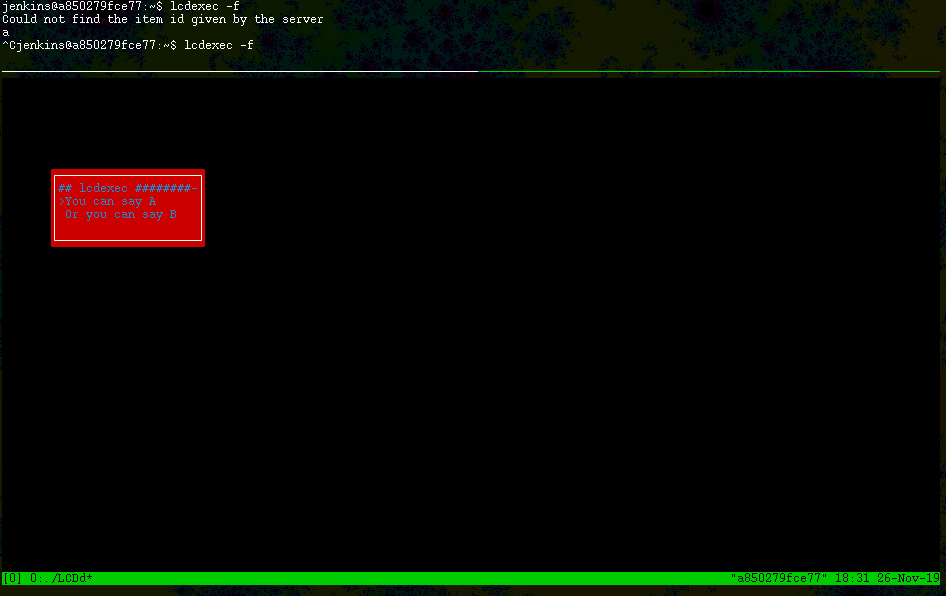
\includegraphics[width=\linewidth]{graphics/lcdexec_menu.png}
  \caption{Menu navigation in LCDd while lcdexec is connected}
\label{fig:lcdexec}
\end{figure}
\FloatBarrier
We see both of our configured menus, and, on selecting the first menu option, we also see that \texttt{a} gets printed in the lcdexec window.
We also see a warning message, that an item id could not be found, which gets printed, when the server has sent an unknown command.

\section{lcdvc}
The lcdvc client can display a system console on a display which is controlled by LCDd.
Our configuration file only contains two assignments, the rest of the 33 lines consist of comments and empty lines.
In the created \acrshort{toml} configuration we set the devices to read from to \texttt{/dev/urandom}.
\begin{Verbatim}[frame=single, fontsize=\small]
kdb set user/sw/lcdproc/lcdvc/#0/current/lcdvc/vcsdevice \
    /dev/urandom
kdb set user/sw/lcdproc/lcdvc/#0/current/lcdvc/vcsadevice \
    /dev/urandom
diff -ws lcdproc/lcdvc.toml .config/lcdvc.toml
31,32c31,32
< vcsdevice="/dev/null"
< vcsadevice="/dev/null"
---
> vcsdevice = "/dev/urandom"
> vcsadevice = "/dev/urandom"
\end{Verbatim}
We see, that the only file differences are the values we changed by \texttt{kdb set} before.
\\\\
When we start LCDd and lcdexec in a \acrshort{tmux} session, we see that lcdexec forwards the stream of \texttt{/dev/urandom} to LCDd.
\FloatBarrier
\begin{figure}[h!]
	\centering
		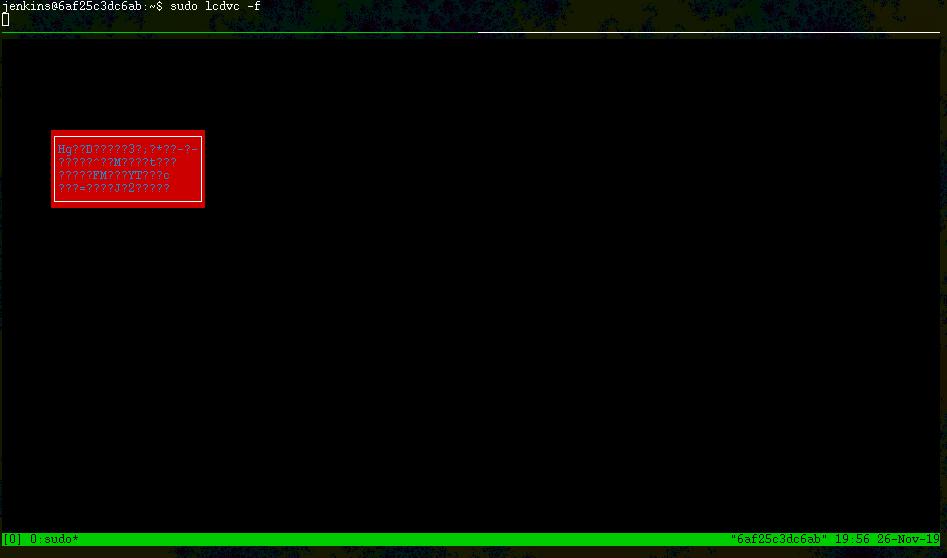
\includegraphics[width=\linewidth]{graphics/lcdvc.png}
  \caption{LCDd receiving \texttt{/dev/random} from lcdexec}
\label{fig:lcdvc}
\end{figure}
\FloatBarrier

\section{Benchmarks}

\subsection{Additional Setup}
For Elektra, we used our fork of Elektra \cite{bauhausforkelektra}.
For LCDproc, we used our fork of Elektra's fork of LCDproc \cite{bauhausforklcdproc}.
\subsubsection{\acrshort{toml}}
\begin{Verbatim}[frame=single, fontsize=\small]
elektra:
    branch 'thesis_bench'
    commit #0052eba6de6d46ec5265fdc01a1fd83046afe104
lcdproc:
    branch 'toml_test'
    commit #adadaaec1ede9a5ecf840020ec5eee5585ecbf29
\end{Verbatim}
\subsubsection{\acrshort{yaml}}
\begin{Verbatim}[frame=single, fontsize=\small]
elektra:
    branch 'thesis_bench'
    commit #0052eba6de6d46ec5265fdc01a1fd83046afe104
lcdproc:
    branch 'bench_yaml'
    commit #e9e9cd97c1a5116214b53bff4649aea00726d37c
\end{Verbatim}

\subsubsection{ni}
\begin{Verbatim}[frame=single, fontsize=\small]
elektra:
    branch 'thesis_bench'
    commit #0052eba6de6d46ec5265fdc01a1fd83046afe104
lcdproc:
    branch 'bench_ni'
    commit #1d06f0c65cd7252bbb4a43aeb7bbd59e6b9118f0
\end{Verbatim}

We benchmarked the \acrshort{toml} plugin against two other Elektra storage plugins, yamlcpp for \acrshort{yaml} (\acrlong{yaml}) and ni for \acrshort{ini}.
To use these plugin for comparision, we had to convert our \acrshort{toml} configuration file used in the previous evaluation into \acrshort{yaml} and \acrshort{ini}.

We also had to disable two required plugins from the yamlcpp plugin, because otherwise we would get an error from Elektra for too many mounted plugins on the start of LCDd.
The disabled plugins were the \texttt{directoryvalue} and the \texttt{base64} plugin.
The \texttt{directoryvalue} plugin would be needed if we wanted to write non-leaf keys into the file (and subsequently, convert them back on reading).
The \texttt{base64} plugin would be needed if we had to handle binary key/values.
For reading the configuration files, neither of those functionalities are need.
For benchmarking purposes, we also modified the LCDd main function, to not execute it's mainloop after initialization, but instead exit the application.
\subsection{Execution}
We benchmarked the three plugins by executing them repeatedly within a python script:
\begin{Verbatim}[frame=single, fontsize=\small]
RUNS = 100
times = []
for _ in range(RUNS):
	start = time.time()
	subprocess.call(["LCDd", "-f"])
	times.append(1000. * (time.time() - start))

avg = sum(times) / RUNS
median = times[round(RUNS/ 2)]
print(f"runs = {RUNS}\navg = {avg}ms\n
    median = {median} ms\nmin = {min(times)} ms\n
    max = {max(times)} ms")
\end{Verbatim}
\subsection{Results}
\FloatBarrier
\begin{table}[!ht]
	\centering
	\begin{tabular}{ccccc}
	\toprule
	plugin & avg & median & min & max \\
	\midrule
	toml 	& 75.03 ms	& 75.46 ms	& 66.01 ms	& 166.86 ms \\
	yamlcpp & 80.72 ms	& 83.55 ms	& 67.32 ms	& 134.60 ms \\
	ni		& 74.16 ms	& 75.28 ms	& 65.89 ms	& 160.39 ms \\
	\bottomrule
	\end{tabular}
	\caption{Benchmarks for LCDd}
	\label{tab:benchmarks}
\end{table}
\FloatBarrier

\section{Discussion}
In this evaluation, we tested not only basic key/value assignments, but also \acrshort{toml} features like tables and table arrays, and even nested arrays, which all could be read and restored correctly.
We could observe that in all four programs of LCDproc, we would get identical files after reading/writing them when ignoring whitespace.
This also means, that no comments got lost or misordered during roundtripping a file.
Only during lcdexec evaluation we got a warning for a missing menu id, but since our configured command got executed anyway, we assumed success. This may be no error attributable to the written plugin.
\\\\
The benchmarks showed, that the reading speed of the plugin can match with two other existing Elektra storage plugins, with the ni plugin being the current default for LCDprocs configuration storage.

\chapter{Future Work}
One thing, that the \acrshort{toml} plugin currently cannot store is Elektra metadata. Other plugins, like \texttt{yamlcpp} and \texttt{ni} already support this feature.
The \texttt{yamlcpp} plugin does this by assigning a special meaning to the value '!elektra/meta', which indicates that the key must be handeled in a different matter \cite{elektrayamlcpp}.
For the \acrshort{toml} plugin we could maybe store metadata info in the comments before key with metadata, also by introducing a special sequence which indicate the presence of metadata.

As an example, a key \texttt{'a'} with a type metakey of value \texttt{unsigned\_short} could look like:
\begin{Verbatim}[frame=single, fontsize=\small]
#!ELEKTRA_META! type=unsigned_short
a = 3
\end{Verbatim}
When reading a file with this special tagged comments, we could differentiate them already at the stage of lexing from normal comments.
However, there is the question of how this would affect the readability of a \acrshort{toml} file, when it contains many many metadata.

Another thing that could be improved in the future, would be a more complete preservation of whitespace characters.
Especially whitespace used as indentation in front of keys/tables/table arrays/array elements would be very nice, since they improve human readability of the file.
We actually tried to preserve this kind of whitespace, but turned it back, since the grammar got too error prone.
When implemented properly, two points need to be taken care of:
On the one side, the bison grammar should emit no reduce/reduce or shift/reduce ambiguities.
On the other side, a valid \acrshort{toml} file should not be invalid because a valid spot for whitespace got overlooked in the grammar.
When we first tried to implement this feature, we struggled with these two problems, which seemed to amplify each other.
If we would eliminate more grammar ambiguities, we would get more files parsed as invalid and vice-versa.

\chapter{Related Work}

In his master's thesis, Markus Raab laid the groundwork for Elektras plugin based structure \cite{raabmaster}.
He also describes the problems that a storage plugin has to solve, like preserving the order of the data in the file or avoiding any loss of information between roundtrips of a file.

A general overview on how to create a parser with both flex and bison can be found in the book written by John Levine \cite{levineflexbison}.
There he also elaborates on which kinds of conflicts can occur when writing a parser with bison and how to resolve them.
He also writes about how to emit useful error messages from within the lexer/parser.

A more theoretical background on how formal languages could be parsed can be found in Stefano Reghizzi's book on formal languages \cite{reghizziformallanguages}.


\chapter{Conclusion}
In this paper, we wanted to verify, if our written \acrshort{toml} plugin reads and writes the LCDproc configuration correctly.
We also wanted to survey, if the plugin puts an unreasonable overhead on the LCDproc startup time.

In our evaluation, we saw that the plugin could handle the configuration needed by LCDproc.
It would do so in both reading and writing direction.
No information got lost when reading / writing different configuration files of LCDproc.
\\\\
Furthermore, the benchmarks showed that it has a decent reading speed of the LCDd configuration file, compared to two other storage plugins.

\backmatter

\listoffigures

\listoftables

% \printindex

\printglossary[type=\acronymtype]

\bibliography{references}{}
\bibliographystyle{plain}

\end{document}
